%%%
%% Testing :: Functional Testing
%%%
\section{Functional Testing}
\label{sec:functional_testing}

%%%
%% Testing :: Functional Testing :: Usability Requirements
%%%
\subsection{Usability Requirements}
\label{sub:test_func_usability}

 \paragraph{Provide a text field for the user to input the cryptic clue to be}
  A text field has been added to the interface to allow the user to enter a cryptic clue. 
\begin{figure}[H]
	\centering
	 
\includegraphics[keepaspectratio=true]{evidence/enterclue.png}
	\caption{Text field to enter clue}
\end{figure}

{\bf Overall:} Fully Implemented

 \paragraph{Provide a drop-down box allowing the user to input the
number of words in the solution, with an initial upper-
limit of 10 words}

 A text field has been provided instead of a drop-down box which allows the user
 to input the number of words as well as the length of the words. The limit on the 
amount of words input by the user has not been implemented, however the user 
can only input words of length up to fifteen. This is because a traditional cryptic 
crossword has a typical size of 15x15.

\begin{figure}[H]
	\centering
	
\includegraphics[keepaspectratio=true]{evidence/dropdown1.png}
	\caption{Attempting to enter a length of sixteen - the red colour signifies it is invalid}
\end{figure}

\begin{figure}[H]
	\centering
	
\includegraphics[keepaspectratio=true]{evidence/dropdown2.png}
	\caption{Attempting to enter two words of length fifteen - the green colour signifies it is valid}
\end{figure}

\begin{figure}[H]
	\centering
	
\includegraphics[keepaspectratio=true]{evidence/dropdown3.png}
	\caption{Attempting to enter three words of valid length with a space and a hyphen - the green 
colour signifies it is valid}
\end{figure}

{\bf Overall:} Alternatively Implemented

\paragraph{Dynamically provide individual text boxes for each word
of the solution, which allow the length of the words to be
specified. Also provide check-boxes between these text-
boxes to define whether they are separated by a space
or a hyphen}

See `Provide a drop-down box allowing the user to input the
number of words in the solution, with an initial upper-
limit of 10 words'.

{\bf Overall:} Alternatively Implemented

\paragraph{Dynamically provide text boxes to represent each char-
acter of each word of the solution, allowing the user to
input any known characters}

Text boxes are dynamically created depending on the values input into 
the `Solution Length' field. 

\begin{figure}[H]
	\centering
	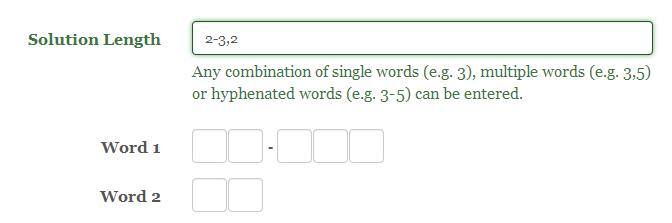
\includegraphics[keepaspectratio=true,scale=0.9]{evidence/dynamicboxes.png}
	\caption{Boxes that have been generated for a solution with the configuration; 2-3,2}
\end{figure}

{\bf Overall:} Fully Implemented

\paragraph{Provide a table of results which allow the user the to
view the possible solutions}

When the results are returned to the user, they are displayed within a table 
underneath the fields containing the users input. 

\begin{figure}[H]
	\centering
	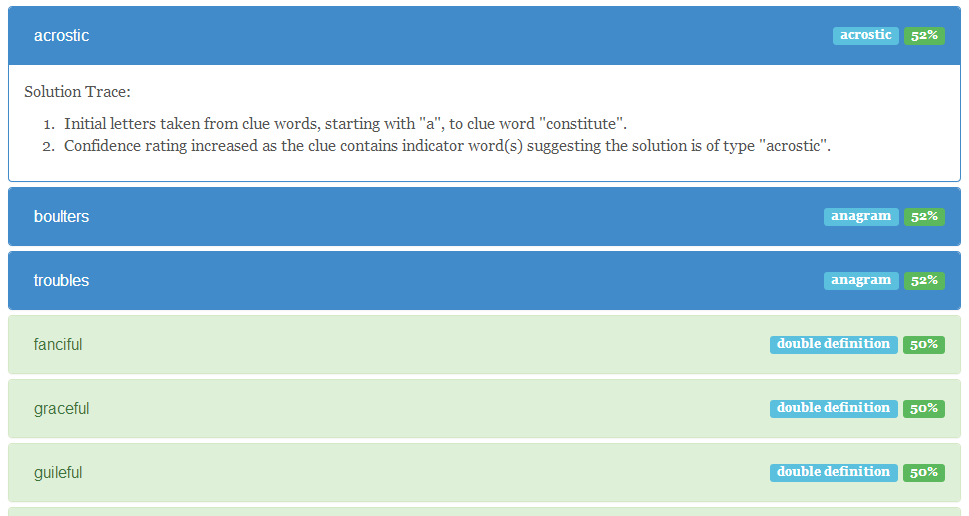
\includegraphics[keepaspectratio=true,scale=0.6]{evidence/listsolutions.png}
	\caption{Results displayed for the clue; `A clever rhyme or subtle teaser I constitute'}
\end{figure}

{\bf Overall:}: Fully Implemented

\paragraph{Alert the user to required fields with red asterisks}
   A design decision was made to change the colour of the label text 
and the outline of the text box if the user clicks `Submit' without filling in
 required fields.

\begin{figure}[H]
	\centering
	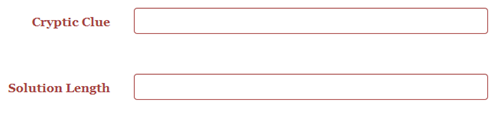
\includegraphics[keepaspectratio=true]{evidence/alert1.png}
	\caption{If the user submits without filling in either required fields}
\end{figure}

\begin{figure}[H]
	\centering
	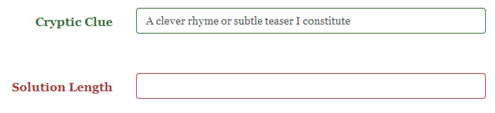
\includegraphics[keepaspectratio=true]{evidence/alert2.png}
	\caption{If the user submits without filling in the length of the solution}
\end{figure}

\begin{figure}[H]
	\centering
	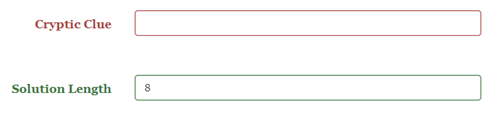
\includegraphics[keepaspectratio=true]{evidence/alert3.png}
	\caption{If the user submits without filling in the clue field}
\end{figure}

{\bf Overall:} Alternatively Implemented

\paragraph{Have a consistent layout avoid unnecessary scrolling}
    All pages within the website have the same colour scheme and fonts 
with an additional consistency with menu items and bars. The web page 
has also been implemented 

\begin{figure}[H]
	\centering
	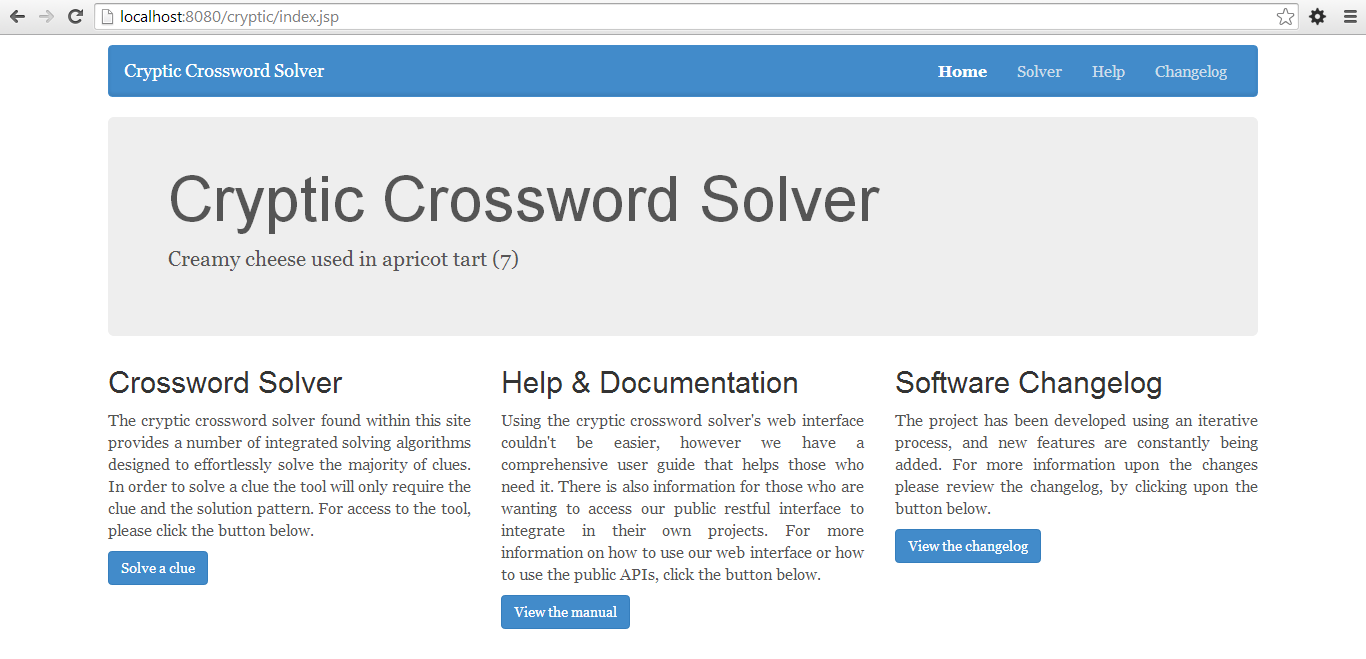
\includegraphics[keepaspectratio=true,scale=0.4]{evidence/scrolling.png}
	\caption{If the user submits without filling in the clue field}
\end{figure}

\begin{figure}[H]
	\centering
	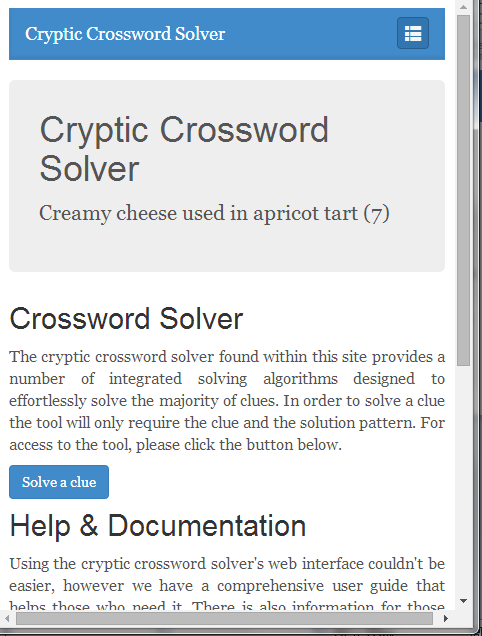
\includegraphics[keepaspectratio=true,scale=0.5]{evidence/scrolling1.png}
	\caption{If the user submits without filling in the clue field}
\end{figure}

{\bf Overall:} Fully Implemented

\paragraph{Alert the user to invalid input through validation checks
with error messages} 
     When the user clicks `Submit' without completing the required fields 
the styling of the label and text fields change colour to red and the page 
does not proceed to pass invalid data to the back end code. 

See `Alert the user to required fields with red asterisks' for evidence'.

{\bf Overall:} Alternatively Implemented 

\paragraph{Provide a confidence rating in the table of possible solutions}

The confidence rating calculated whilst retrieving possible solutions is displayed 
alongside the solution.

\begin{figure}[H]
	\centering
	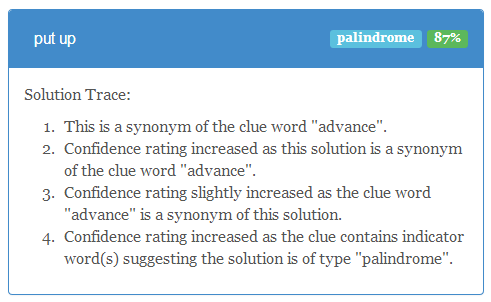
\includegraphics[keepaspectratio=true]{evidence/confidence.png}
	\caption{Confidence ratings displayed with the solutions returned}
\end{figure}

{\bf Overall:} Fully Implemented

\paragraph{Allow the user to select a proposed solution in the corresponding table and mark this as correct}

{\bf Overall:} Not Implemented

\paragraph{Display help buttons to indicate to the user the purpose
and use of each control}

{\bf Overall:} Alternatively Implemented

\paragraph{Provide a button to submit the user input to the appli-
cation for processing}

A submit button has been provided for the user to click when they have input 
the clue itself and the clues length. 

\begin{figure}[H]
	\centering
	
\includegraphics[keepaspectratio=true]{evidence/submit.png}
	\caption{Submit button for user to click}
\end{figure}

{\bf Overall:} Fully Implemented

\paragraph{Provide a group of radio buttons for the user to select
the clue's orientation in its containing crossword}

{\bf Overall:} Not Implemented

\paragraph{Provide a text box to input the clue's number within its
containing crossword}
 
{\bf Overall:} Not Implemented

\paragraph{Provide mechanisms to accommodate for users with dif-
ficulties, such as colour-blindness or poor eyesight}
    
{\bf Overall:} Partially Implemented